\subsection{Adhesion of Metal Oxide Interfaces}
\begin{frame}{
    Adhesion in FeBCC/Fe\textsubscript{3}O\textsubscript{4}
    interface 
  }

  \begin{onlyenv}<1>
    Separating the parts of the interface it is
    possible to obtain energy vs separation curves 
    from DFT calculations.
    Then the forces can be obtained from interface 
    potential models!
  \end{onlyenv}
  \begin{center}
  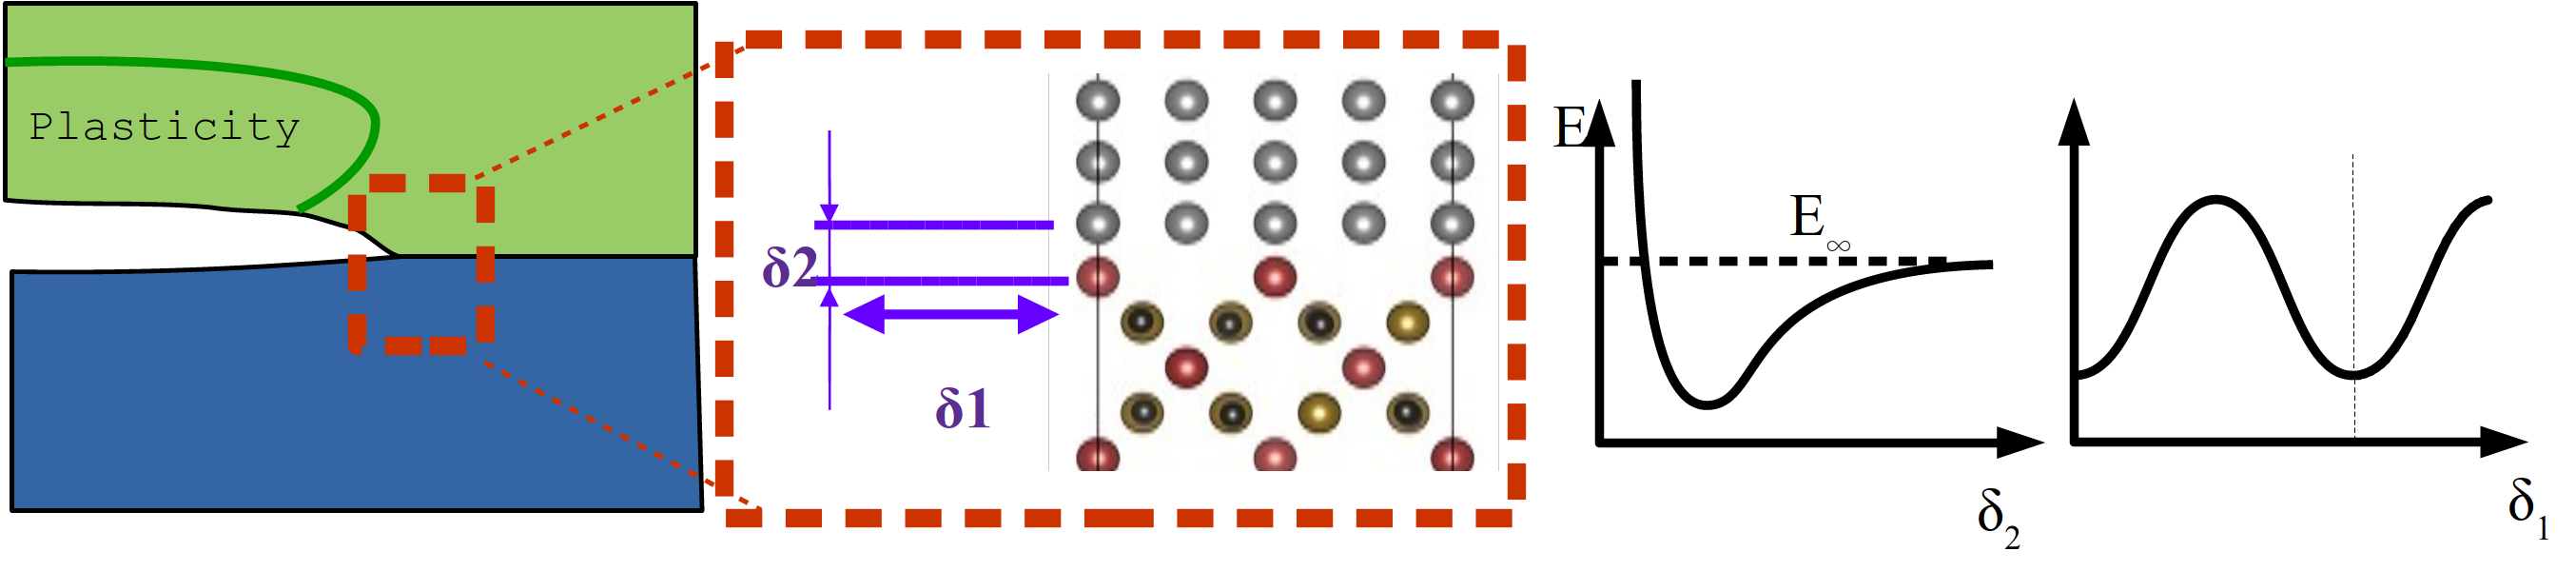
\includegraphics[height=0.3\textheight]{/home/mariano/CuadernoTrabajo/CV/SLI/02-CurrentResearch/Adhesion_Scheme.png}
  \end{center}
\begin{onlyenv}<2->
\begin{columns}
  \column{0.3\textwidth}
  \scalebox{0.4}{\parbox{\textwidth}{
\begin{gather*}
  \tilde{L}_{\delta_1}{}={}
  \frac{E_{ad}}{W_{sep}}{}={}
  \exp{\left(  \frac{\delta_2}{\hat{\delta} } \right)}
  \sum_{i=0} ^{i_{max}} \left(1 + \beta \right) ^i
   \left[ -1 + 
   f (\delta_1) \left( 1 + \beta \right) ^i
   \right]
   \alpha _i
   \left(
   \frac{\delta_2}{\hat{\delta}}
   \right) ^i 
   \\
   \quad
   T_1 \left(\delta_1
   ,\delta_2 \right) = - \frac{\partial W}{\partial \delta _1}
   \quad
   \\
   \quad
   T_2 \left(\delta_1 ,\delta_2 \right) = -\frac{\partial W}{\partial \delta_2}
   \quad
\end{gather*}
  }}
  \column{0.3\textwidth}
    \begin{center}
    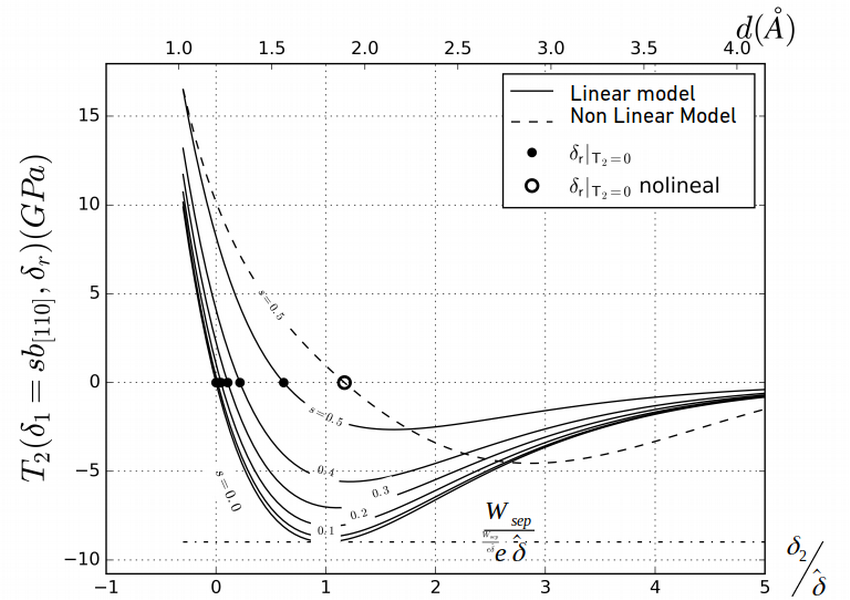
\includegraphics[height=0.4\textheight]{/home/mariano/CuadernoTrabajo/CV/SLI/02-CurrentResearch/T1.png}
    \end{center}
  \column{0.3\textwidth}
    \begin{center}
    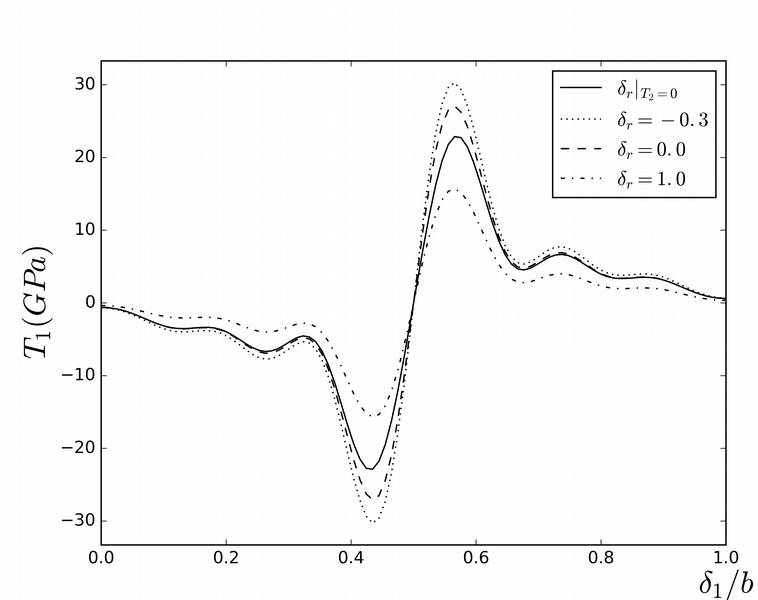
\includegraphics[height=0.4\textheight]{/home/mariano/CuadernoTrabajo/CV/SLI/02-CurrentResearch/T2.png}
    \end{center}
\end{columns}
\end{onlyenv}
\end{frame}
